\documentclass[margin,line]{res}

\usepackage{graphicx}
\usepackage{float}
\usepackage{tabularx}
\usepackage{hyperref}
\hypersetup{
  colorlinks   = true, %Colours links instead of ugly boxes
  urlcolor     = blue, %Colour for external hyperlinks
  linkcolor    = blue, %Colour of internal links
  citecolor   = red %Colour of citations
}

\oddsidemargin -.5in
\evensidemargin -.5in
\textwidth=6.0in
\itemsep=0in
\parsep=0in
% if using pdflatex:
\setlength{\pdfpagewidth}{\paperwidth}
\setlength{\pdfpageheight}{\paperheight} 

\newenvironment{list1}{
  \begin{list}{\ding{113}}{%
      \setlength{\itemsep}{0in}
      \setlength{\parsep}{0in} \setlength{\parskip}{0in}
      \setlength{\topsep}{0in} \setlength{\partopsep}{0in} 
      \setlength{\leftmargin}{0.17in}}}{\end{list}}
\newenvironment{list2}{
  \begin{list}{$\bullet$}{%
      \setlength{\itemsep}{0in}
      \setlength{\parsep}{0in} \setlength{\parskip}{0in}
      \setlength{\topsep}{0in} \setlength{\partopsep}{0in} 
      \setlength{\leftmargin}{0.2in}}}{\end{list}}


\begin{document}

\name{Daobilige Su \vspace*{.1in}}

\begin{resume}

%%%%%%%%%%%%
\section{\sc Personal Information}
\vspace{.05in}
\begin{tabularx}{\textwidth}{X r}
Gender: Male & Date of Birth:10-09-1987 \\ 
Nationality: China (Australian Permanent Residence) \\
Australian Centre for Robotics,      &  +61(02)-93519181 \\            
The University of Sydney,   & sudao2020@outlook.com\\
J18, 8 Little Queen St, Chippendale, NSW 2008, Australia  & \\%{\it E-mail:}  paciorek@stat.cmu.edu\\       
%  & \\%{\it WWW:} www.stat.cmu.edu/\verb+~+paciorek \\     
\end{tabularx}



%%%%%%%%%%%%
\section{\sc Research Interests}
Field Robotics for Precision Agriculture and Livestock, SLAM, Deep Learning for Robot Vision, Autonomous Navigation and Robot Audition


%%%%%%%%%%%%
\section{\sc Current Occupation}
\begin{tabularx}{\textwidth}{X r}
%\href{http://www.uts.edu.au}{{\bf University of Sydney}}, Sydney, Australia  
{\bf PostDoc Research Associate}, &May, 2017 - present\\
\end{tabularx}
%{\em Department of Statistics} 
\vspace*{-.1in}
\begin{list1}
\item[] \href{https://www.sydney.edu.au/engineering/our-research/robotics-and-intelligent-systems/australian-centre-for-robotics.html}{Australian Centre for Robotics (ACFR)}, \\%\\ {\it Expected:} Jan. 2017
\href{https://sydney.edu.au/}{{The University of Sydney}}, Sydney, Australia
\begin{list2}
\vspace*{.05in}
\item Research Topic:  ``Agricultural Robotics for Vegetable Breeding : Digital Phenotyping and Digital Twin Leads'' 
\item Supervisor: \href{http://sydney.edu.au/engineering/people/salah.sukkarieh.php}{Prof. Salah Sukkarieh} %(Director Research and Innovation of ACFR, Fellow of \href{https://www.atse.org.au/}{Australian Academy of Technological Sciences and Engineering}, CEO of \href{https://agerris.com/}{Agerris}) %Fellow of Australian Academy of Technological Sciences and Engineering (ATSE)%, \href{http://sydney.edu.au/engineering/people/james.underwood.php}{Dr. James Underwood}
\end{list2}
\end{list1}
%%%%%%%%%%%%

%%%%%%%%%%%%
\section{\sc Previous Occupation}
\begin{tabularx}{\textwidth}{X r}
%\href{http://www.uts.edu.au}{{\bf University of Sydney}}, Sydney, Australia  
{\bf Associate Professor}, &Sep, 2020 - Apr, 2025\\
\end{tabularx}
%{\em Department of Statistics} 
\vspace*{-.1in}
\begin{list1}
\item[] Dept. of Mechatronic Eng., \href{http://coe.cau.edu.cn/}{College of Eng.}, \\%\\ {\it Expected:} Jan. 2017
\href{http://en.cau.edu.cn/}{{China Agricultural University (CAU)}}, Beijing, China
\end{list1}
\begin{figure}[H]
  \centering
  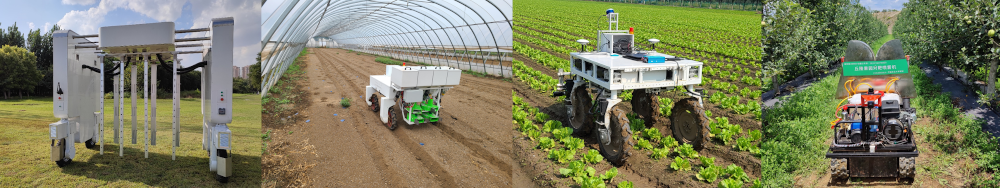
\includegraphics[width=0.99\columnwidth]{./figs/cau_robots_smallsize.png}
  %\caption{The architecture of non-bottleneck-1D block.}
  \label{fig:cau_robots}
\end{figure}

\begin{tabularx}{\textwidth}{X r}
%\href{http://www.uts.edu.au}{{\bf University of Sydney}}, Sydney, Australia  
{\bf PostDoc Research Associate}, &Mar, 2017 - Apr, 2020\\
\end{tabularx}
%{\em Department of Statistics} 
\vspace*{-.1in}
\begin{list1}
\item[] \href{https://sydney.edu.au/engineering/our-research/robotics-and-intelligent-systems/australian-centre-for-field-robotics.html}{Australian Centre for Filed Robotics (ACFR)}, \\%\\ {\it Expected:} Jan. 2017
\href{https://sydney.edu.au/}{{The University of Sydney}}, Sydney, Australia
\begin{list2}
\vspace*{.05in}
\item Research Topic:  ``Intelligent Perception Systems for Agriculture and the Environment'' 
%\item Dissertation Topic:  ``Hierarchical Models for Multiple Ratings
%  in Performance-Based\\ \hspace*{1.23in} Student Assessments.'' 
\item Supervisor: \href{http://sydney.edu.au/engineering/people/salah.sukkarieh.php}{Prof. Salah Sukkarieh} %(Director Research and Innovation of ACFR, Fellow of \href{https://www.atse.org.au/}{Australian Academy of Technological Sciences and Engineering}, CEO of \href{https://agerris.com/}{Agerris}) %Fellow of Australian Academy of Technological Sciences and Engineering (ATSE)%, \href{http://sydney.edu.au/engineering/people/james.underwood.php}{Dr. James Underwood}
\item \textbf{Robots worked on}: \href{https://confluence.acfr.usyd.edu.au/display/AGPub/Our+Robots}{Ladybird, RIPPA, Digital Farmhand and Shrimp} (\href{https://sydney.edu.au/engineering/our-research/robotics-and-intelligent-systems/australian-centre-for-field-robotics/agriculture-and-the-environment.html}{alternative link})
\end{list2}
\end{list1}

\begin{figure}[H]
  \centering
  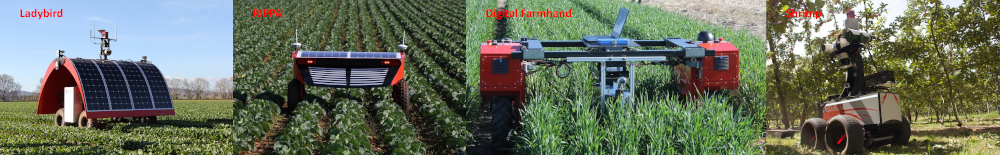
\includegraphics[width=0.99\columnwidth]{./figs/ladybird_rippa_digitalfarmhand_shrimp_smallsize.png}
  %\caption{The architecture of non-bottleneck-1D block.}
  \label{fig:ladybird_rippa_digitalfarmhand_shrimp}
\end{figure}
%%%%%%%%%%%%


%%%%%%%%%%%%
\section{\sc Education}

\begin{tabularx}{\textwidth}{X r}
\href{http://www.uts.edu.au}{{\bf University of Technology Sydney (UTS)}}, Sydney, Australia  &Mar, 2013 - Mar, 2017\\
\end{tabularx}
%{\em Department of Statistics} 
\vspace*{-.1in}
\begin{list1}
\item[] Ph.D. Candidate on Robotics at \href{http://www.cas.uts.edu.au}{Centre for Autonomous System}%\\ {\it Expected:} Jan. 2017
\begin{list2}
\vspace*{.05in}
\item Dissertation Topic:  ``Robotic Sound Source Mapping using Microphone Arrays'' 
%\item Dissertation Topic:  ``Hierarchical Models for Multiple Ratings
%  in Performance-Based\\ \hspace*{1.23in} Student Assessments.'' 
\item Supervisor: \href{http://www.uts.edu.au/staff/jaime.vallsmiro}{A/Prof. Jaime Valls Miro}
\item Co-supervisor:  \href{http://www.uts.edu.au/staff/teresa.vidalcalleja}{Dr. Teresa Vidal Calleja}
\end{list2}
\end{list1}

\begin{tabularx}{\textwidth}{X r}
\href{http://emaro.irccyn.ec-nantes.fr/}{{\bf EMARO} (European Master on Advanced RObotics)} &Oct, 2010 - Oct, 2012\\
\end{tabularx}
%{\em Department of Mathematics and Statistics} 
\vspace*{-.1in}
\begin{list1}
\item[] University of Genova, Italy (Oct, 2011 - Oct, 2012)
\begin{list2}
\vspace*{.05in}
\item Master of Automation, GPA: 92/100
\end{list2}
\begin{list2}
\vspace*{.05in}
\item Master thesis at Keio University, Japan (Apr, 2012 - Sep, 2012)\\
Thesis topic: Designing Real-Time Robot Audition System\\
Thesis supervisor: Prof. Nozumo Hamada
\end{list2}
\end{list1}
\begin{list1}
\item[] Warsaw University of Technology, Poland (Oct, 2010 - Jul, 2011)
\begin{list2}
\vspace*{.05in}
\item Master of Automation and Robotics, GPA: 81.5/100
\end{list2}
\end{list1}

\begin{tabularx}{\textwidth}{X r}
\href{http://www.zju.edu.cn/english/}{{\bf Zhejiang University}}, Hangzhou, China   &Sep, 2006 - Jul, 2010\\
\end{tabularx}
%{\em Department of Mathematics and Statistics} 
\vspace*{-.1in}
\begin{list1}
\item[] Bachelor of Mechatronic Engineering, GPA: 3.63/4.0 (last 2 years:3.76/4.0)
\end{list1}



%%%%%%%%%%%%



%%%%%%%%%%%%
\section{\sc Selected Publications}
%Paciorek, C.J., J.S. Risbey, V. Ventura, and R.D.Rosen. 2002. Multiple indices of Northern Hemisphere Cyclone
%Activity, Winters 1949-1999. Journal of Climate 15:1573-1590.
%
%Paciorek, C.J., R. Condit, S.P. Hubbell, and R.B. Foster.  2000.
%The demographics of resprouting in tree and shrub species of a moist
%tropical forest.  Journal of Ecology 88:765-777.
%
%Paciorek, C.J., B.R. Moyer, R.A. Levin, and S.L. Halpern.  1995.
%Pollen consumption by hummingbird flower mite {\it Proctolaelaps
%  kirmsei} and possible fitness effects on {\it Hamelia patens}.
%Biotropica 27:258-262.  (author order determined by lot)
% ($^{\#}$ indicates the first author/authors (with equal contributions), * indicates the corresponding author/authors)\\
% \textbf{Journal Publications}

\begin{enumerate}

% Su, Daobilige, He Kong, Salah Sukkarieh, and Shoudong Huang. "Necessary and sufficient conditions for observability of SLAM-Based TDOA sensor array calibration and source localization." IEEE Transactions on Robotics 37, no. 5 (2021): 1451-1468.
\item \textbf{D. Su}$^{\#}$, H. Kong*, S. Sukkarieh, and S. Huang, ``Necessary and sufficient conditions for observability of SLAM-Based TDOA sensor array calibration and source localization'', {\it IEEE Transactions on Robotics}, vol. 37 no. 5, p. 1451-1468, 2021. (2022 \textbf{IF 6.835})

% Wang, Jiang, Yuanzheng He, Daobilige Su, Katsutoshi Itoyama, Kazuhiro Nakadai, Junfeng Wu, Shoudong Huang, Youfu Li, and He Kong. "SLAM-based Joint Calibration of Multiple Asynchronous Microphone Arrays and Sound Source Localization." IEEE Transactions on Robotics (2024).
\item J. Wang$^{\#}$, Y. He, \textbf{D. Su}, K. Itoyama, K. Nakadai, J. Wu, S. Huang, Y. Li, and H. Kong*, ``SLAM-based Joint Calibration of Multiple Asynchronous Microphone Arrays and Sound Source Localization'', {\it IEEE Transactions on Robotics} (Online)), 2024. (2023 \textbf{IF 9.4})

% S. Wang, D. Su, Y. Jiang, Y. Tan, Y. Qiao, S. Yang, Y. Feng, and N. Hu, "Fusing vegetation index and ridge segmentation for robust vision based autonomous navigation of agricultural robots in vegetable farms," Computers and Electronics in Agriculture, vol. 213, p. 108235, 2023. (2022 IF 8.3)
% \item S. Wang$^{\#}$, \textbf{D. Su*}, Y. Jiang, Y. Tan, Y. Qiao, S. Yang, Y. Feng, and N. Hu, ``Fusing vegetation index and ridge segmentation for robust vision based autonomous navigation of agricultural robots in vegetable farms'', {\it Computers and Electronics in Agriculture}, vol. 213, p. 108235, 2023. (2022 \textbf{IF 8.3})

% \item W. Li$^{\#}$, S. Jiang, S. Yang, H. Feng, W. Liu, Y. Zheng*, Y. Tan, and \textbf{D. Su}, ``Leaf-density estimation for fruit-tree canopy based on wind-excited audio'', {\it Journal of Field Robotics}, vol. 41 no. 5, p. 1469-1479, 2024. (2022 \textbf{IF 8.3})

% N. Hu, D. Su, S. Wang, X. Wang, H. Zhong, Z. Wang, Y. Qiao, and Y. Tan, "Segmentation and tracking of vegetable plants by exploiting vegetable shape feature for precision spray of agricultural robots," Journal of Field Robotics, Online, 2023. (2022 IF 8.3)
\item N. Hu$^{\#}$,  \textbf{D. Su*}, S. Wang, X. Wang, H. Zhong, Z. Wang, Y. Qiao, and Y. Tan, ``Segmentation and tracking of vegetable plants by exploiting vegetable shape feature for precision spray of agricultural robots'', {\it Journal of Field Robotics}, vol. 41 no. 3, p. 570-586, 2024. (2022 \textbf{IF 8.3})

%Xue, Tengfei, Yongliang Qiao, He Kong, Daobilige Su, Shirui Pan, Khalid Rafique, and Salah Sukkarieh. "One-shot Learning-based Animal Video Segmentation." IEEE Transactions on Industrial Informatics (2021).
\item T. Xue$^{\#}$, Y. Qiao*, H. Kong, \textbf{D. Su}, S. Pan, K. Rafique, and S. Sukkarieh, ``One-shot Learning-based Animal Video Segmentation'', {\it IEEE Transactions on Industrial Informatics}, vol. 18 no. 6, p. 3799-3807, 2022. (2022 \textbf{IF 11.648})



%Su, Daobilige, Yongliang Qiao, He Kong, and Salah Sukkarieh. "Real time detection of inter-row ryegrass in wheat farms using deep learning." Biosystems Engineering 204 (2021): 198-211.
% \item \textbf{D. Su}$^{\#}$, Y. Qiao*, H. Kong, and S. Sukkarieh, ``Real time detection of inter-row ryegrass in wheat farms using deep learning'', {\it Biosystems Engineering}, vol. 204, p. 198-211, 2021. (2022 \textbf{IF 5.002})

%Su, Daobilige, He Kong, Yongliang Qiao, and Salah Sukkarieh. "Data augmentation for deep learning based semantic segmentation and crop-weed classification in agricultural robotics." Computers and Electronics in Agriculture 190 (2021): 106418.
\item \textbf{D. Su}$^{\#}$, H. Kong*, Y. Qiao, and S. Sukkarieh, ``Data augmentation for deep learning based semantic segmentation and crop-weed classification in agricultural robotics'', {\it Computers and Electronics in Agriculture}, vol. 190, p. 106418, 2021. (2022 \textbf{IF 6.757})

% %Kong, He, Mao Shan, Daobilige Su, Yongliang Qiao, Abdullah Al-Azzawi, and Salah Sukkarieh. "Filtering for systems subject to unknown inputs without a priori initial information." Automatica 120 (2020): 109122.
% \item H. Kong$^{\#}$*, M. Shan, \textbf{D. Su}, Y. Qiao, A. Al-Azzawi, and S. Sukkarieh, ``Filtering for systems subject to unknown inputs without a priori initial information'', {\it Automatica}, vol. 120, p. 109122, 2020. (2019 IF \textbf{5.541})

% %Qiao, Yongliang, He Kong, Cameron Clark, Sabrina Lomax, Daobilige Su, Stuart Eiffert, and Salah Sukkarieh. "Intelligent perception for cattle monitoring: A review for cattle identification, body condition score evaluation, and weight estimation." Computers and Electronics in Agriculture 185 (2021): 106143.
% \item Y. Qiao$^{\#}$, H. Kong, C. Clark, S. Lomax, \textbf{D. Su}, S. Eiffert, and S. Sukkarieh, ``Intelligent perception for cattle monitoring: A review for cattle identification, body condition score evaluation, and weight estimation'', {\it Computers and Electronics in Agriculture}, vol. 185, p. 106143, 2021. (2021 \textbf{IF 5.565})

% %Brown, Jasper, Daobilige Su, He Kong, Salah Sukkarieh, and Eric C. Kerrigan. "Improved noise covariance estimation in visual servoing using an autocovariance least-squares approach." Mechatronics 68 (2020): 102381.
% \item J. Brown$^{\#}$, \textbf{D. Su}, H. Kong*, S. Sukkarieh, and E. Kerrigan. ``Improved Noise Covariance Estimation in Visual Servoing Using an Autocovariance Least-squares Approach'', \textit{Mechatronics}, vol. 68, p. 102381, 2020. (2020 IF \textbf{2.992})

% %Su, Daobilige, Teresa Vidal-Calleja, and Jaime Valls Miro. "Asynchronous microphone arrays calibration and sound source tracking." Autonomous Robots 44, no. 2 (2020): 183-204.
% \item {\bf D. Su}$^{\#}$*, T. Vidal Calleja, and J. Valls Miro, ``Asynchronous microphone arrays calibration and sound source tracking'', {\it Autonomous Robots}, vol. 44 no. 2, p. 183-204, 2020. (2022 \textbf{IF 4.262})

% % Wang, Mengmeng, Yong Liu, Daobilige Su, Yufang Liao, Lei Shi, and Jinhong Xu. "Accurate and Real-time 3D Tracking for the Following Robots by Fusing Vision and Ultra-sonar Information." IEEE/ASME Transactions on Mechatronics (2018).
% \item M. Wang$^{\#}$, Y. Liu*, {\bf D. Su}, Y. Liao, L. Shi, J. Xu, and J. Valls Miro, ``Accurate and Real-time 3D Tracking for the Following Robots by Fusing Vision and Ultrasonar Information'', in {\it IEEE/ASME Transactions on Mechatronics}, vol. 23 no. 3, p. 997-1006, 2018. (2018 \textbf{IF 3.936})
% \end{enumerate}

% \textbf{Conference Publications}
% \begin{enumerate}

% \item Z. He$^{\#}$, J. Wang, \textbf{D. Su}, K. Nakadai, J. Wu, S. Huang, Y. Li, and H. Kong*. ``Observability analysis of graph SLAM-based joint calibration of multiple microphone arrays and sound source localization'', in \textit{2023 IEEE/SICE International Symposium on System Integration (SII 2023)}, pp. 1-8. IEEE, 2023.

% \item Y. Qiao$^{\#}$*, \textbf{D. Su}, H. Kong, S. Sukkarieh, S. Lomax, and C. Clark. ``Data Augmentation for Deep Learning based Cattle Segmentation in Precision Livestock Farming'', in \textit{2020 IEEE International Conference on Automation Science and Engineering (CASE 2020)}, 2020.

% \item Y. Qiao$^{\#}$*, \textbf{D. Su}, H. Kong, S. Sukkarieh, S. Lomax, and C. Clark. ``BiLSTM-based Individual Cattle Identification for Automated Precision Livestock Farming'', in \textit{2020 IEEE International Conference on Automation Science and Engineering (CASE 2020)}, 2020.

% %Qiao, Yongliang, Daobilige Su, He Kong, Salah Sukkarieh, Sabrina Lomax, and Cameron Clark. "Individual Cattle Identification Using a Deep Learning Based Framework." IFAC-PapersOnLine 52, no. 30 (2019): 318-323.
% \item Y. Qiao$^{\#}$*, \textbf{D. Su}, H. Kong, S. Sukkarieh, S. Lomax, and C. Clark. ``Individual Cattle Identification Using a Deep Learning Based Framework'', in {\it AgriControl 2019}, p. 318-323, 2019.

% % Brown, Jasper, Daobilige Su, He Kong, Salah Sukkarieh, and Eric Kerrigan. "Improved Noise Covariance Estimation in Visual Servoing Using an Autocovariance Least-squares Approach."
% %The 12th IFAC Conference on Control Applications in Marine Systems, Robotics, and Vehicles (CAMS 2019) and the first workshop on Robot Control (WROCO 2019)
% \item J. Brown$^{\#}$, \textbf{D. Su}, H. Kong, S. Sukkarieh, and E. Kerrigan. ``Improved Noise Covariance Estimation in Visual Servoing Using an Autocovariance Least-squares Approach'', in \textit{Joint 12th IFAC Conference on Control Applications in Marine Systems, Robotics, and Vehicles (CAMS 2019) and the first workshop on Robot Control (WROCO 2019)}, 2019. ({\bf Best Paper Award Finalist}).

% % Wang, Min, Holger Voos, and Daobilige Su. "Robust Online Obstacle Detection and Tracking for Collision-Free Navigation of Multirotor UAVs in Complex Environments." In 2018 15th International Conference on Control, Automation, Robotics and Vision (ICARCV), pp. 1228-1234. IEEE, 2018.
% \item M. Wang$^{\#}$, H. Voos, and {\bf D. Su}, ``Robust Online Obstacle Detection and Tracking for Collision-free Navigation of Multirotor UAVs in Complex Environments'', in {\it 2018 15th International Conference on Control Automation Robotics \& Vision (ICARCV 2018)}, p. 1228-1234, 2018.

% % KANZHI WU, Teng Zhang*, Daobilige Su, Shoudong Huang, Gamini Dissanayake
% % An Invariant-EKF VINS Algorithm for Improving Consistency
% % Wu, Kanzhi, Teng Zhang, Daobilige Su, Shoudong Huang, and Gamini Dissanayake. "An invariant-EKF VINS algorithm for improving consistency." In Intelligent Robots and Systems (IROS), 2017 IEEE/RSJ International Conference on, pp. 1578-1585. IEEE, 2017.
% \item K. Wu$^{\#}$, T. Zhang$^{\#}$, {\bf D. Su}, S. Huang, and G. Dissanayake, ``An Invariant-EKF VINS Algorithm for Improving Consistency'', in {\it 2017 IEEE/RSJ International Conference on Intelligent Robots and Systems (\textbf{IROS 2017})}, p. 1578-1585, 2017.

% % Su, Daobilige, Teresa Vidal-Calleja, and Jaime Valls Miro. "Towards real-time 3D sound sources mapping with linear microphone arrays." In Robotics and Automation (ICRA), 2017 IEEE International Conference on, pp. 1662-1668. IEEE, 2017.
\item {\bf D. Su}$^{\#}$*, T. Vidal Calleja, and J. Valls Miro, ``Towards Real-Time 3D Sound Sources Mapping with Linear Microphone Arrays'', in {\it 2017 IEEE International Conference on Robotics and Automation (\textbf{ICRA 2017})}, p. 1662-1668, 2017.
% %2017. 
% (Affiliated Video: \\ \href{https://youtu.be/Ry_i3kmvlHM}{{https://youtu.be/Ry\_i3kmvlHM}}, Open source code: \\ \href{https://github.com/daobilige-su/SSM_LinearArray}{{https://github.com/daobilige-su/SSM\_LinearArray}})

% Wang, Mengmeng, Daobilige Su, Lei Shi, Yong Liu, and Jaime Valls Miro. "Real-time 3D human tracking for mobile robots with multisensors." In Robotics and Automation (ICRA), 2017 IEEE International Conference on, pp. 5081-5087. IEEE, 2017.
\item M. Wang$^{\#}$, {\bf D. Su}, L. Shi, Y. Liu, and J. Valls Miro, ``Real-time 3D Human Tracking for Mobile Robots with Multisensors'', in {\it 2017 IEEE International Conference on Robotics and Automation (\textbf{ICRA 2017})}, p. 5081-5087, 2017.

% \item {\bf D. Su}$^{\#}$*, T. Vidal Calleja, and J. Valls Miro, ``Split Conditional Independent Mapping for Sound Source Localisation with Inverse-Depth Parametrisation'', in {\it 2016 IEEE/RSJ International Conference on Intelligent Robots and Systems (\textbf{IROS 2016})}, p. 2000-2006, 2016. 
% % (Affiliated Video: \href{https://youtu.be/QyqY2eIX1wk}{{https://youtu.be/QyqY2eIX1wk}})

% \item {\bf D. Su}$^{\#}$*, K. Nakamura, K. Nakadai, and J. Valls Miro, ``Robust Sound Source Mapping using Three-layered Selective Audio Rays for Mobile Robots'', in {\it 2016 IEEE/RSJ International Conference on Intelligent Robots and Systems (\textbf{IROS 2016})}, p. 2771-2777, 2016.

% \item {\bf D. Su}$^{\#}$*, T. Vidal Calleja, and J. Valls Miro, ``Simultaneous asynchronous microphone array calibration and sound source localisation'', in {\it 2015 IEEE/RSJ International Conference on Intelligent Robots and Systems (\textbf{IROS 2015})}, p. 5561-5567, 2015.

% \item {\bf D. Su}$^{\#}$*, J. Valls Miro, and T. Vidal Calleja, ``Graph-SLAM Based Calibration of an Embedded Asynchronous Microphone Array for Outdoor Robotic Target Tracking'', in {\it Assistive Robotics: Proceedings of the 18th International Conference on CLAWAR 2015}, p. 641-648, 2015. ({\bf Best Paper Award Finalist}).

% \item {\bf D. Su}$^{\#}$*, J. Valls Miro, and T. Vidal Calleja, ``Real-time sound source localisation for target tracking applications using an asynchronous microphone array'', in {\it 2015 IEEE 10th Conference on Industrial Electronics and Applications (ICIEA 2015)}, p. 1261-1266, 2015.

% \item {\bf D. Su}$^{\#}$*, J. Valls Miro, and T. Vidal Calleja, ``Modelling in-pipe acoustic signal propagation for condition assessment of multi-layer water pipelines'', in {\it 2015 IEEE 10th Conference on Industrial Electronics and Applications (ICIEA 2015)}, p. 545-550, 2015. ({\bf Best Paper Award Finalist}).

% \item {\bf D. Su}$^{\#}$*, N. Ulapane, and B. Wijerathna, ``An acoustic sensor based novel method for 2D localization of a robot in a structured environment'', in {\it 2015 IEEE 10th Conference on Industrial Electronics and Applications (ICIEA 2015)}, p. 2024-2029, 2015.

% \item {\bf D. Su}$^{\#}$*, and J. Valls Miro. ``An ultrasonic/RF GP-based sensor model robotic solution for indoors/outdoors person tracking'', in {\it 2014 13th International Conference on Control Automation Robotics \& Vision (ICARCV 2014)}, p. 1662-1667, 2014.

% \item T. Vidal Calleja$^{\#}$*, {\bf D. Su}, F. De Bruijn, and J. Valls Miro, ``Learning spatial correlations for Bayesian fusion in pipe thickness mapping'', in {\it 2014 IEEE International Conference on Robotics and Automation (\textbf{ICRA 2014})}, p. 683-690, 2014.

% \item J. Valls Miro$^{\#}$*, J. Rajalingam, T. Vidal Calleja, F. de Bruijn, R. Wood, D. Vitanage, N. Ulapane, B. Wijerathna and {\bf D. Su}, ``A live test-bed for the advancement of condition assessment and failure prediction research on critical pipes'', in {\it Proceedings of the Leading-Edge Strategic Asset Management Conference (LESAM13)}. 2013.

% \item {\bf D. Su}$^{\#}$, M. Sekikawa, K. Nakazawa and N. Hamada, ``Novel scheme of real-time direction finding and tracking of multiple speakers by robot-embedded microphone array'', in {\it the 1st International Conference on Robot Intelligence Technology and Applications (RITA 2012)}, 2012.

\end{enumerate}

% %%%%%%%%%%%%
% \section{\sc Teaching Experience}

% \begin{tabularx}{\textwidth}{X r}
% {\bf Undergraduate Level Teaching} & Sept, 2020 - now, China Agricultural University\\
% \end{tabularx}
% \begin{itemize}
% \item[] \textbf{Fundamentals of Control Theory}, covers basic concepts of complex variable function, control system modeling, time domain analysis of LTI system, frequency domain analysis of LTI system, stability analysis of LTI system, classic regulators for LTI system, etc.

% % \vspace*{-1.5mm}
% \item[] \textbf{Autonomous Mobile Robot}, covers mechanical design and motion models for various mobile robots, common sensors and their modeling, signal processing, localization and mapping, path planning and motion planning, etc.

% % \vspace*{-1.5mm}
% \item[] \textbf{Machine Learning (Lab)}, covers practical case studies for object detection, semantic and instance segmentation, optical character recognition, pose estimation, video classification, deep reinforcement learning for robot control, etc.

% % \vspace*{-1.5mm}
% \item[] \textbf{Robot SLAM and Navigation (Lab)}, covers practical case studies for visual SLAM and 3D Lidar SLAM, path planning and motion planning, etc.
% \end{itemize}

% \begin{tabularx}{\textwidth}{X r}
% {\bf Graduate Level Teaching} & Sept, 2022 - now, China Agricultural University\\
% \end{tabularx}
% \begin{itemize}
% \item[] \textbf{Robot Modeling and Programming}, covers lectures and labs for robot modeling and simulation with Gazebo and CoppeliaSim, ROS system structure, ROS topic, message, service, param, action, common tools in ROS, and various case studies, including robotic SLAM, autonomous navigation, and development process of an orchard spray robot, etc.

% % \vspace*{-1.5mm}
% \item[] \textbf{Agricultural Robots}, covers lectures and labs for common sensors for agricultural robots, current state-of-the-art methods for common perception tasks such as object detection, semantic and instance segmentation, point cloud segmentation, point cloud registering, visual SLAM, 3D Lidar base SLAM methods, classic path planning and motion planning methods, and several case studies, etc.
% \end{itemize}

% %%%%%%%%%%%%
% \section{\sc Academic Experience}
% \begin{tabularx}{\textwidth}{X r}
% {\bf Academic Engagement} & Feb, 2015\\
% \end{tabularx}
% \begin{itemize}
% \item[] \textbf{Associate Editor} for Journals: Precision Agriculture (Elsevier) and Frontiers in Plant Science (Frontiers). \textbf{Associate Editor} for IROS 2021-2022.
% \end{itemize}

% \begin{tabularx}{\textwidth}{X r}
% {\bf Summer School} & Feb, 2015\\
% \end{tabularx}
% \begin{itemize}
% \item[] \href{http://rp-www.cs.usyd.edu.au/~mlss/}{2015 Machine Learning Summer School}, University of Sydney, Australia

% \vspace*{-2.5mm}
% \item[] Bayesian Inference and MCMC, Structured Prediction, Bayesian Nonparametrics, Natural Language Processing, Deep Learning, etc.
% \end{itemize}

% \begin{tabularx}{\textwidth}{X r}
% {\bf Summer School} & Jul, 2011\\
% \end{tabularx}
% \begin{itemize}
% \item[] \href{http://www.asl.ethz.ch}{ASL (Autonomous Systems Lab)}, ETH Zurich, Switzerland

% \vspace*{-2.5mm}
% \item[] Design, Perception, and Control for Autonomous Micro Aerial Vehicles
% \end{itemize}

% %%%%%%%%%%%%
% \section{\sc Work Experience}

% \begin{tabularx}{\textwidth}{X r}
% {\bf Internship} & May, 2015 - Sep, 2015\\
% \end{tabularx}
% \begin{itemize}
% \item[] \href{http://www.jp.honda-ri.com/english}{Honda Research Institute, Japan (HRI-JP)}

% \vspace*{-2.5mm}
% \item[] Supervisors: Dr. Keisuke Nakamura and Prof. Kazuhiro Nakadai
% \end{itemize}

% \begin{tabularx}{\textwidth}{X r}
% {\bf Internship} & Feb, 2010 - Jun, 2010\\
% \end{tabularx}
% \begin{itemize}
% \item[] Bosch Power Tools (China) Co., Ltd.

% \vspace*{-2.5mm}
% \item[] Manufacturing Manager Assistant
% \end{itemize}

% %%%%%%%%%%%%
% \section{\sc Honors and Awards} 
% \begin{itemize}

% \item {\bf CAU Excellent Talent} title from China Agricultural University, 2020.

% \vspace*{-2.5mm}
% \item {\bf UTS IRS} %(International Research Scholarship) 
% scholarship and {\bf UTS FEIT Faculty} scholarship for PhD study at UTS, 2013-2016.

% \vspace*{-2.5mm}
% \item {\bf Erasmus Mundus Scholarship} for Master study as EMARO, funded by European Union, Approx. 10 scholarships available for applications from all over the world (outside Europe), 2010-2012.

% \vspace*{-2.5mm}
% \item {\bf Academic Excellent Scholarship} by Zhejiang University, China.

% \vspace*{-2.5mm}
% \item {\bf Tuition Wave Scholarship} 4 times in Academic year 2006-2010 by Zhejiang University, China.

% \vspace*{-2.5mm}
% \item {\bf National Stipend} 4 times in Academic year 2006-2010, funded by Chinese Ministry of Education

% \vspace*{-2.5mm}
% \item 1st Prize in {\bf Mechatronic System Design Competition} in Zhejiang Uni. Oct, 2009-Feb, 2010

% \vspace*{-2.5mm}
% \item 1st Prize out of 1620 teams from 159 universities/colleges/institutes in {\bf National Energy Saving and Emission Reduction Competition} Feb, 2009-Sep, 2009


% \end{itemize}

% %%%%%%%%%%%%
% \section{\sc Computer Skills} 
% \begin{list2}
% \item {\bf Programming}: Matlab, C/C++ and Python (good), Java and Unix/Linux kernel programming (acquired). \\

% \item {\bf Robotics Libraries}: ROS1 and ROS2, OpenCV, TensorFlow, PyTorch and CoppeliaSim (good), OpenGL, QT and PCL (acquired).\\

% \item {\bf Hardware Design}: AutoCAD, Solidworks and ProE(good), Altium Designer, Pspice and Multisim (acquired).\\

% \item {\bf Simulation}: COMSOL Multi Physics (good), AnSys, Gambit and Fluid (acquired) \\
% \end{list2}

%%%%%%%%%%%%
\section{\sc Computer Skills} 
\begin{list2}

\item {\bf Associate Editor for IROS 2022}: serves as an associate Editor for 2021 IEEE/RSJ International Conference on Intelligent Robots and Systems (IROS 2022). \\

\item {\bf Organizer for IROS 2022 workshop}: serves as a co-organizer for IROS 2022 Special Session: Robotics in Agriculture and Livestock Farming Systems.\\

\item {\bf Associate Editor for IROS 2021}: serves as an associate Editor for 2021 IEEE/RSJ International Conference on Intelligent Robots and Systems (IROS 2021). \\

\item {\bf Associate Editor for Precision Agriculture}: serves as an associate Editor for Springer journal Precision Agriculture, specialized in the robotics and artificial intelligence in agriculture. \\

\item {\bf Associate Editor for Frontiers in Plant Science}: serves as an associate Editor for Frontiers in Plant Science, specialized in the robotics and artificial intelligence in agriculture. \\

\end{list2}

% %%%%%%%%%%%%
% \section{\sc Language Skills} 
% English: Professional (TOEFL ibt 108/120)\\
% Chinese and Mongolian: Native\\
% German and Japanese: Beginner




%\vspace{-.3cm}
%{\em Graduate Student} \hfill {\bf August, 1998 - present}\\
%Includes current Ph.D.~research, Ph.D.~and Masters level coursework and
%research/consulting projects.
%
%%\vspace{-.1cm}
%{\em Instructor} \hfill {\bf May - June, 2002}\\
%Co-taught graduate level course for the Master of Science in
%Computational Finance program.  Shared responsibility for lectures, exams,
%homework assignments, and  grades.  
%\vspace*{.05in}  
%\begin{list2}
%\item 46-731 Probability and Statistics, Summer 2002.
%\end{list2}


%%\vspace{-.1cm}
%{\em NSF VIGRE Teaching Fellow} \hfill {\bf January - May, 2001}\\
%Head teaching assistant.   
%Duties included  shared administrative responsibilities with faculty
%instructor, fielding of all student inquiries, and oversight of
%graduate student teaching assistants and graders.
%\vspace*{.05in}  
%\begin{list2}
%\item 36-217 Probability Theory and Random Processes, Spring 2001.
%\end{list2}
%
%%\vspace{-.1cm}
%{\em Teaching Assistant} \hfill {\bf August, 2001  - present}\\
%Duties at various times have included 
%office hours and leading weekly computer lab exercises.


   


%%%%%%%%%%%%
%\section{\sc Papers in preparation}
%
%Ventura, V., C.J. Paciorek, and J.S. Risbey.  Controlling the proportion of falsely-rejected hypotheses when conducting multiple tests with geophysical data.
%
%Ickes, K., C.J. Paciorek, and S. Thomas.  Effects of wild pigs on
%forest demographic processes in Malaysia.
%
%

%%%%%%%%%%%%
%\section{\sc Conference Presentations}
%Paciorek, C.J., J.S. Risbey, V. Ventura, and R.D.Rosen.  2001.  Changes in Northern Hemisphere winter storm activity (1949-1999) based
%on a comparison of cyclone indices.  8th International Meeting on
%Statistical Climatology, Luneberg, Germany, March, 2001.
%
%Paciorek, C.J. and R. Rosenfeld.  2000.  Minimum classification error
%training in exponential language models.  2000 Spring Transcription
%Workshop, College Park, Maryland.
%\vspace*{-.25in}  
%\begin{verbatim}http://www.nist.gov/speech/publications/tw00/html/abstract.htm#cp1-50\end{verbatim}
%
%
%

%%%%%%%%%%%%
%\section{\sc Professional Experience}
%{\bf Bureau of Transportation Statistics, U.S. Department of
%  Transportation}, Washington, District of Columbia USA
%
%\vspace{-.3cm}
%{\em Summer researcher} \hfill {\bf May, 2000 - August, 2000}\\
%Carried out several consulting projects, including modelling of
%injuries to cadavers in crash test experiments, analysis of airline
%delay data, and advice on analysis of airline economics data.
%
%{\bf Abt Associates}, Bethesda, Maryland USA
%
%\vspace{-.3cm}
%{\em Associate Programmer Analyst and Research Assistant} \hfill {\bf
%  October, 1994 - August, 1996}\\
%Researcher and computer model developer for U.S. EPA Regulatory Impact
%Analysis of Section 403 Lead Paint Hazard Rule.  Other projects
%included database analysis, literature reviews, and cost-benefit analysis.







\end{resume}
\end{document}




